This chapter describes first the overall structure of the project, its technical requirements (which can and later be used as part of the evaluation) and then dives into the implementation of individual modules.

I refer to this project by its name \textsl{graffs}.
A working version is published on GitHub\footnote{\url{https://github.com/jjurm/graffs}} along with its source code.


\section{Overview}

The purpose of this project is to develop a methodology and tool, i.e. a framework, to help study graph metrics, and empirically analyse their robustness in particular.

\begin{figure}[p!]
    \centering
    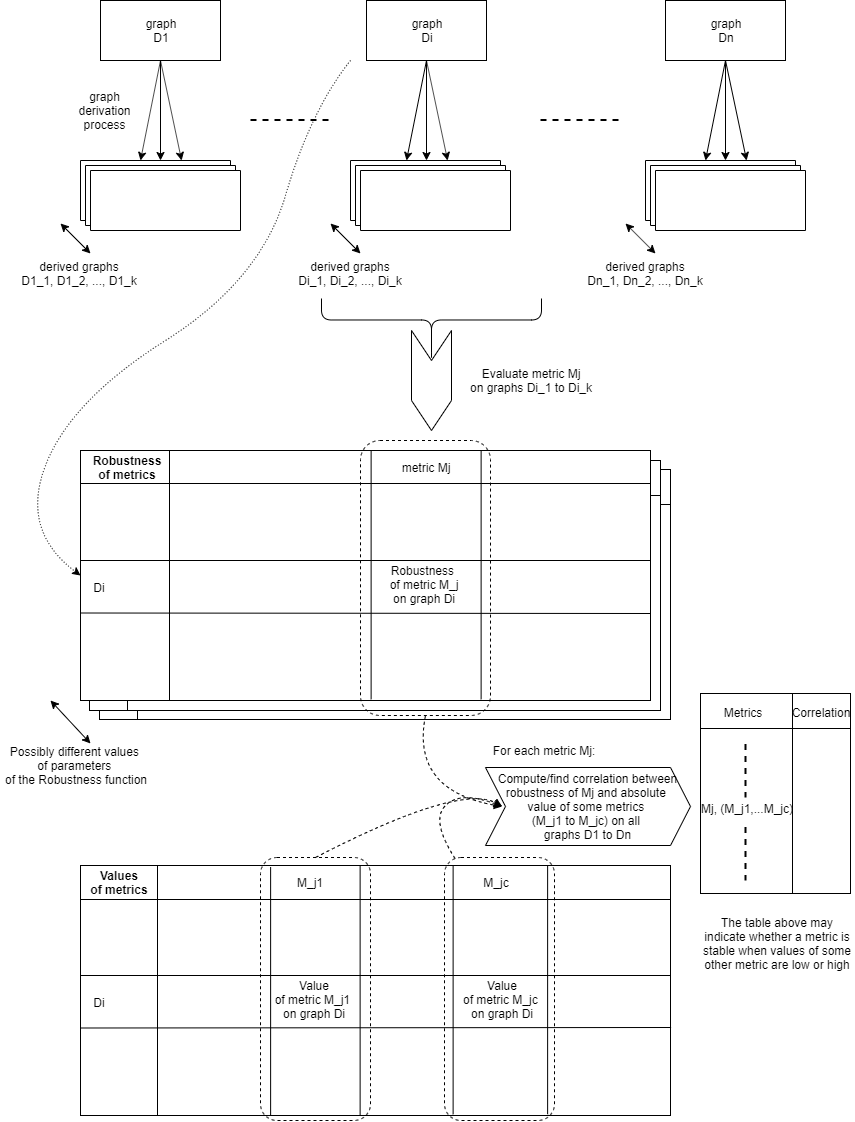
\includegraphics[width=16cm]{proposal_diagram1.png}
    \caption{An illustration of the evaluation process.\\ \todo{make this diagram up to date, using notation from~\nameref{ch:preparation}}.
    A generator is used to generate perturbed graphs from each input dataset.
    Each metric from a chosen set of metrics is evaluated on all petrurbed graphs.
    From those results, robustness values of each metric on each dataset are calculated using each chosen robustness measures.
    This is referred to in the project as the ``Main pipeline''}
    \label{fig:overview_prop_diagram}
\end{figure}


\graffs is a command-line tool written in Kotlin\citeneeded that can load/store datasets of different formats, generate perturbed graphs, evaluate metrics, and calculate robustness values. \autoref{fig:overview_prop_diagram} is a diagram explaining the natural flow of the program, i.e. the \textsl{main pipeline} where we start with graph datasets and end up with deductions about each metric's


\section{Design goals}\label{sec:design-goals}

The following are technical requirements I set for the project.
Overall, I aim this tool to be reusable for similar projects, either by directly invoking the compiled binary, or by using it as a dependency, or by forking and extending it.

\todo{specify who is the target user of \graffs}

\subsection{Supported features}

\graffs supports the following features:

\begin{enumerate}
    \item Store, load input graphs in various formats, and represent them in a unified memory structure
    \item Run algorithms that compute metrics on graphs
    \item Generate graphs by applying perturbations to given input graphs
    \item Run experiments by evaluating metrics on generated graphs in a systematic manner
    \item Calculate robustness of metrics based on experiments
    \item Possibly, produce visual output from the results
\end{enumerate}

\subsection{Scalability}

According to The Paper~\cite{Bozhilova2019}, calculating natural connectivity for a single node for a graph with ~7000 nodes takes ~88 seconds on a standard computer.
In one of my toy examples, calculating average betweenness centrality of ~2500 nodes took ~8 minutes on my personal computer.
Thus, assuming computing a (computation-heavy) metric(s) on an input graph of average size 5000 nodes takes ~30 minutes, the pure computation time suggested by the~\nameref{ch:proposal} would take the following time on a standard personal computer (approximated in the order of magnitude)
\[(\sim 6\ \text{datasets}) \times (\sim 6\ \text{metrics}) \times (\sim 50\ \text{derived graphs}) \times (\sim 30\ \text{minutes}) \approx 38\ \text{days}\]

For this reason, one of the goals is to make the program efficient and runnable on a supercomputer, utilising the power of multi-core systems for parallel execution.

\subsection{Reproducibility}

It is important for all results in research to be reproducible.
By \textsl{reproducibility} of \graffs I mean the guarantee that one can exactly reproduce any results produced by the program.
I.e. when the program is run two times with the same input and hyper-parameters, it must produce the same output.
And by \textsl{the same output} I mean producing the same images, tables, numbers up to a bit-wise match.

This is a challenge in all the following areas:
\begin{itemize}
    \item \textbf{Stochastic processes}

    Methods based on stochastic processes or randomness must be reproducible.
    An example of a stochastic method are graph generators.

    These can be made reproducible done by generating all randomness starting off with a given seed for the generator.

    \item \textbf{Resolving ties}

    Methods that are not inherently stochastic but require pseudo-randomness to resolve ties must also be reproducible.
    An example is generating a visual layout for graphs such as in \autoref{fig:simple_graph}.
    This layout algorithm needs to resolve ties when starting with a graph where nodes have no position.

    Again, a solution is to base such flow on an input seed.

    \item \textbf{External factors}

    Unpredictability introduced by the operating system and other external factors must be accounted for, so that the program still produces the same results even if run on a different supported machine, in a different environment.
    This is more challenging in a concurrent environment when it must be made sure the produced output does not depend on any factors such as uncertainty and unpredictability of the OS's thread scheduler.

    These issues are resolved using a robust programming language and concurrency synchronisation approaches.
\end{itemize}

\subsection{Flexibility}

The program must be flexible enough, in particular the following:
\begin{enumerate}
    \item Usable on all widely used machines and operating systems
    \item Accepting input datasets (and any input parameters) in common formats
    \item As a library, it must provide modular access to individual parts of the program, so that it is easy to use \graffs as a dependency in future projects of a similar kind
\end{enumerate}


\section{Architecture}

In this section I explain major decisions about the program, such as the choice of the Kotlin language, and Git, Gradle tools.

\subsection{Kotlin language}

I used the programming language \textbf{Kotlin}, mainly for the following reasons.
It is by nature similar to Java and can be used together with other Java code in a single project.
Performance-wise, Kotlin is comparable to Java.
\begin{itemize}
    \item Concise, reducing the amount of boilerplate code
    \item Safer, preventing a significant number of errors
    \item IDE-friendly, allowing the IDE to help with software engineering
    \item Employs functional programming paradigms\cite{Bonev}
    \item Compiles to Java byte code and so preserves other important benefits of Java: Object-Oriented, multi-threaded, platform-independent, secure and easily extensible.
\end{itemize}

Using Kotlin in the project still allows including any libraries written in Java, as Kotlin compiler compiles \texttt{.kt} files to Java-bytecode \texttt{.class} files.
Kotlin has most of its concepts and features adopted from Java, such as classes, polymorphism, inheritance, so these concepts I will freely use in this work.

Kotlin has a number of advanced features such as improved type safety and reduced boilerplate code\cite{JemerovKotlinAction2017}.
There is one notable feature of Kotlin: properties.
Properties are an abstraction of fields and getters/setters in classes and help decouple the implementation of the class from its interface even more.
In UML diagrams in this work , instead of presenting fields and methods of each class, listed are methods and properties (in this order).

\todo{diagram of Kotlin, Gradle, Git, server}

\subsection{Version Control System}

The source code of the \graffs tool is stored in a Git repository, which keeps track of all code changes and allows understanding how code changed over time as well as restoring previous versions.

The repository can be found at \url{https://github.com/jjurm/graffs}.

\subsection{Build automation}

The project uses Gradle\citeneeded for project management.
Split into different modules, Gradle also helps to keep the structure well defined and manages builds of each module separately (which is called a multi-project build in Gradle).

Project configuration rules are set up using the \texttt{build.gradle} files (one in the root directory, then one within each module) with a number of plugins to facilitate the following and more:
\begin{enumerate}
    \item Defines the structure of the project, such as the directories for each module, and source and build directories of each
    \item Automates the process of compiling the code, running tests and producing deployable \texttt{jar}s
    \item Manages and automatically downloads dependencies
    \item Helps with version numbering
    \item Generates HTML API documentation for Kotlin and Java classes
\end{enumerate}


\todo{maybe put all subsections below somewhere at the end of Implementation}

\subsection{Computing cluster}\label{sec:computing_cluster}

I used a remote high-performance computing facility provided by the Systems Research Group (\url{https://www.cl.cam.ac.uk/research/srg/}), sponsored by Dr Andrew Moore (\url{andrew.moore@cl.cam.ac.uk}).

In particular, I worked with the server \texttt{rio.cl.cam.ac.uk} with \todo{include computing characteristics}.

\subsubsection{Setting up the cluster}

\subsection{Project modules}

The project is structured in the following modules, using multi-project builds in Gradle:
\begin{itemize}
    \item \texttt{core} - APIs for structures, metrics, generators, etc., as well as the core data model for storing data in the database
    \item \texttt{storage} - accessing and loading graphs/datasets stored in the filesystem
    \item \texttt{generators} - graph generators
    \item \texttt{metrics} - graph metrics
    \item \texttt{robustness} - robustness measures
    \item \texttt{cli} - code for command-line interface
\end{itemize}

\todo{diagram of code structure + modules + packages}


\section{Data model}

The \graffs tool uses a number of libraries to represent graphs in memory, define a data model, and store data in a relational database.
This section explains how the data of the program is persisted.

The following entities highligh the main concept, and there are some more entities stored in the database.
\begin{itemize}[topsep=5pt]
    \item \textsl{Graph} storing its nodes, edges (and their attributes)
    \item \textsl{Graph generator} is an object capable of producing a number of graphs, given a dataset.
    \item \textsl{Experiment} is a description of a computational task involving:
    \begin{enumerate}[topsep=5pt]
        \item generating graphs from given input datasets using a given graph generator
        \item evaluating a given set of metrics on all generated graphs
        \item evaluate given robustness measures on all metrics over all datasets of the experiment
    \end{enumerate}
\end{itemize}

A user can create and manage \textsl{graph generators} and \textsl{experiments} using the command line interface (see \autoref{sec:cli}).

\subsection{Using GraphStream}

Graphs in memory are stored and manipulated by the GraphStream library\cite{DutotGraphStreamToolBridging2007}, a \enquote{Java library for the modeling and analysis of dynamic graphs. You can generate, import, export, measure, layout and visualize them}

\begin{figure}[ht]
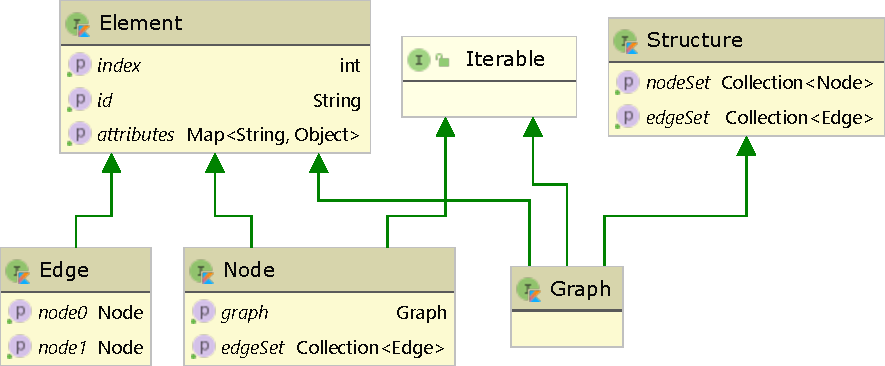
\includegraphics[width=0.65\linewidth]{graphstream_diagram.pdf}
\caption{A simplified diagram of key interfaces from the GraphStream library}
\label{fig:graphstream_diagram}
\end{figure}


The library is based around the \texttt{Graph} interface, which provides access to \texttt{Node}s and \texttt{Edge}s of each graph.
The most relevant interfaces are illustrated in \autoref{fig:graphstream_diagram} (heavily simplified).
The interfaces also provide methods for changing graphs (adding/removing nodes, edges, attributes, etc.).
In practice the library's interfaces contain many more links and methods (e.g. for handling directed graphs) that are not relevant in the context of this project.

For evaluation of robustness, we need to be able to compare (ranks of) values of a specific node between two or more generated graphs, therefore we need to be able to preserve mapping of nodes of a generated graph to nodes in the original dataset (see definition~\ref{def:graph_matching}).
Note that all \texttt{Element}s (i.e. \texttt{Node}s, \texttt{Edge}s and even \texttt{Graph}s) have an \texttt{id} field which will be used for matching nodes between base and perturbed graphs.
This makes evaluation of robustness more straightforward as ranks of nodes in respect to a given metric can be compared across multiple graphs generated from the same base graph.

The GraphStream library also provides a solid base for numerous features in this project such as loading graph files, storing them in various formats, and visualisations.
The GraphStream library allows working with dynamic graphs (changing over time), my project only uses static graphs.
The library also contains an implementation of some graph metrics.

\parspace

The \texttt{Graph} object from the GraphStream library stores (references) all nodes and edges, along with attributes.
In my project, if a metric has been evaluated on a graph, the metric's value for each node is stored as the \texttt{Node}'s attribute, all contained within the \texttt{Graph} object.
The attribute key is given my the metric name.

\subsection{Relational model}

Data of the \graffs tool such as generated graphs, evaluated metrics, robustness measure results as well as any user-defined hyper-parameters are stored in a relational database system.
The Java Persistence API (JPA)~\cite{BiswasJavaPersistenceAPI2016} provides an abstraction for accessing relational data from Java, Hibernate~\cite{ElliottHibernateDeveloperNotebook2004,BauerJavaPersistenceHibernate2015} is a framework that implements the inteface.
I used specifically the H2 database engine\cite{MuellerH2DatabaseEngine2006} as the underlying storage for Hibernate.
This abstraction is later illustrated in \autoref{fig:orm_kotlin_h2_diagram}.

\begin{figure}
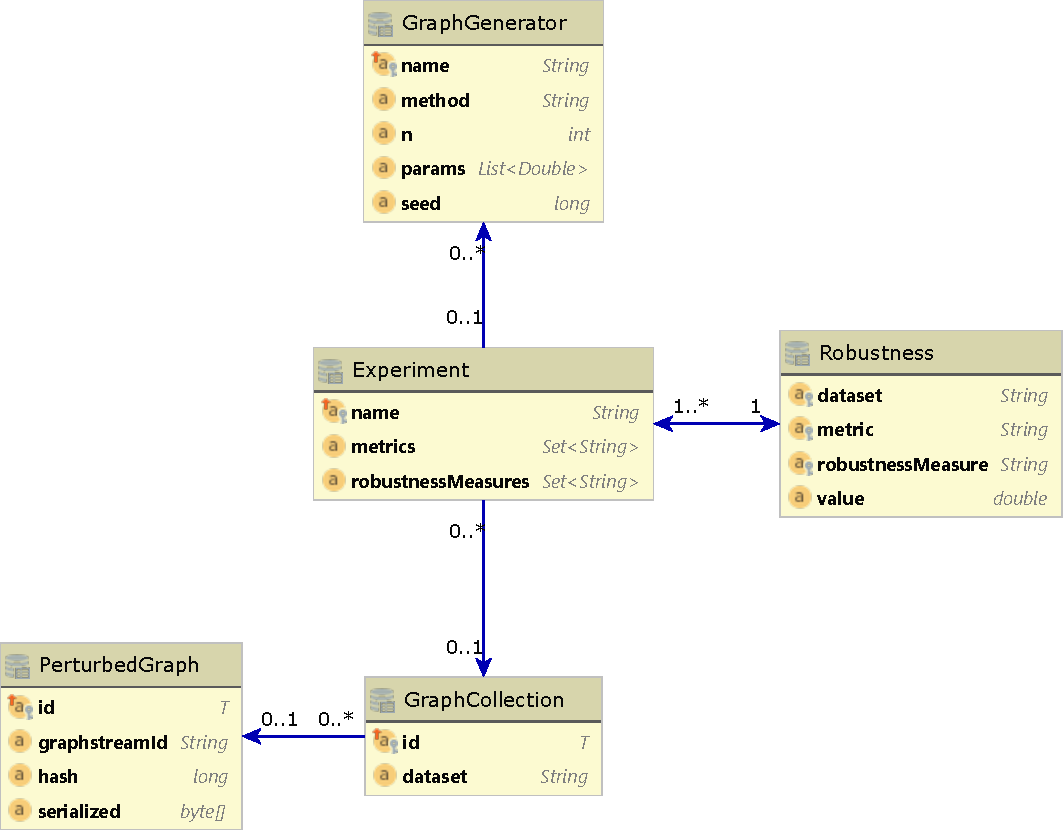
\includegraphics[width=0.9\linewidth]{data_model_diagram.pdf}
\caption{Data model diagram showing \textsl{persistence schema}, i.e. entities stored in the database.
The arrows indicate \textsl{association} links, i.e. ``has a'' or ``refers to'' relationships.
The diagram is created from the Java Persistence API schema inferred from the source code.}
\label{fig:data_model_diagram}
\end{figure}


\autoref{fig:data_model_diagram} shows the entities that the program persists in the database, as explained below.
Named entities (\texttt{Experiment}, \texttt{GraphGenerator}) are those that the user creates and later refers to with their name.
\begin{description}
    \item[\texttt{PerturbedGraph}]
    stores a serialised version of the \texttt{Graph} object, inclucing all so-far evaluated metric values of nodes, and possibly a weight associated with each edge (for scored networks).
    It also stores metadata, such as a hash which distinguishes the graph from other graphs beloging to the same \texttt{GraphCollection} coming from the same graph generator.
    For example in the case graphs are generated by \hyperref[sec:randomly_removing_edges]{randomly removing edges}, the starting seed value of the generator of the particular graph is used as its hash.

    \item[\texttt{GraphCollection}]
    represents an (ordered) collection of \texttt{PerturbedGraph}s.
    It also keeps track of which datasets the graphs were generated from.

    \item[\texttt{GraphGenerator}]
    is an entity that stores user-defined rules for generating graphs from a dataset.
    Once a graph generator is defined and created, it can universally be used on multiple input datasets.
    The parameters of a generator include the name of the method to use (such as \texttt{linear-thresholding}), number of perturbed graphs to generate from each input dataset, seed, and any additional numeric parameters specific to each generator.

    \item[\texttt{Experiment}]
    an entity that encapsulates a concept of evaluating multiple \textsl{robustness measures} of multiple \textsl{metrics} on multiple \textsl{datasets}, using a specific graph generator.
    With an existing generator, the user defines an experiment, which can then be evaluated (see \autoref{sec:main_pipeline}).

    \item[\texttt{Robustness}]
    an entity that stores a single result of evaluating a \textsl{robustness measure} of a \textsl{metric}, on a set of perturbed graphs originating from a certain \textsl{dataset}.
    These robustness values each belong to its parent \texttt{Experiment}.
    Note (\autoref{fig:data_model_diagram}) that the four fields \texttt{experiment}, \texttt{dataset}, \texttt{metric}, \texttt{robustnessMeasure} together form the primary key.
\end{description}

\subsection{Java Persistence API}

The Java Persistence API\cite{BiswasJavaPersistenceAPI2016} (JPA) is an API specification for management of relational data in Java.
It describes ways in Java to specify schemas of relational databases and an interface to manage and access data of a relational model (i.e. entities in tables, relations, first-order logic).
\textsl{Persistence} is an abstract term referring to accessing, managing, and storing entities.

The Hibernate framework~\cite{ElliottHibernateDeveloperNotebook2004,BauerJavaPersistenceHibernate2015}, an object-relational mapping tool, provides a concrete implementation of JPA.
I use Hibernate as the intermediate layer between the \texttt{core} module of \graffs and the underlying H2 database that is completely abstracted away from the \graffs code (\autoref{fig:orm_kotlin_h2_diagram}).

\begin{figure}[ht]
    \vspace*{0.3cm}

    \tikzset{every picture/.style={line width=0.75pt}} %set default line width to 0.75pt

    \begin{tikzpicture}[x=0.75pt,y=0.75pt,yscale=-1,xscale=1]
%uncomment if require: \path (0,182); %set diagram left start at 0, and has height of 182

%Flowchart: Document [id:dp21196524185892507]
        \draw  [fill={rgb, 255:red, 215; green, 213; blue, 186 }  ,fill opacity=1 ][line width=1.5] [blur shadow={shadow xshift=2.25pt,shadow yshift=-1.5pt, shadow blur radius=1.5pt, shadow blur steps=4 ,shadow opacity=45}] (27.93,54) -- (130,54) -- (130,115.84) .. controls (66.2,115.84) and (78.96,138.14) .. (27.93,123.71) -- cycle ;
%Image [id:dp8157383933237885]
        \draw (76.96,73.21) node  {
\includegraphics[width=55.44pt,height=12.32pt]{Kotlin_logo_wordmark.png}};
%Shape: Diamond [id:dp1258210345503794]
        \draw  [fill={rgb, 255:red, 247; green, 244; blue, 209 }  ,fill opacity=1 ][line width=1.5] [blur shadow={shadow xshift=2.25pt,shadow yshift=-1.5pt, shadow blur radius=1.5pt, shadow blur steps=4 ,shadow opacity=45}] (314,54.96) -- (368.93,93.75) -- (314,132.54) -- (259.07,93.75) -- cycle ;
%Image [id:dp807711922850731]
        \draw (312.63,92.23) node  {
\includegraphics[width=71.69pt,height=19.9pt]{Hibernate_logo_a.png}};
%Flowchart: Magnetic Disk [id:dp301549321862431]
        \draw  [fill={rgb, 255:red, 16; green, 33; blue, 255 }  ,fill opacity=1 ][line width=1.5] [blur shadow={shadow xshift=2.25pt,shadow yshift=-1.5pt, shadow blur radius=1.5pt, shadow blur steps=4 ,shadow opacity=45}] (522,72.08) -- (522,113.38) .. controls (522,119.52) and (505.45,124.5) .. (485.03,124.5) .. controls (464.61,124.5) and (448.06,119.52) .. (448.06,113.38) -- (448.06,72.08)(522,72.08) .. controls (522,78.22) and (505.45,83.2) .. (485.03,83.2) .. controls (464.61,83.2) and (448.06,78.22) .. (448.06,72.08) .. controls (448.06,65.94) and (464.61,60.96) .. (485.03,60.96) .. controls (505.45,60.96) and (522,65.94) .. (522,72.08) -- cycle ;
%Image [id:dp005669783415606533]
        \draw (496.46,97.63) node  {
\includegraphics[width=36.81pt,height=20.15pt]{h2-logo.png}};
%Flowchart: Connector [id:dp7113910887207657]
        \draw  [color={rgb, 255:red, 0; green, 0; blue, 0 }  ,draw opacity=1 ][fill={rgb, 255:red, 86; green, 99; blue, 255 }  ,fill opacity=1 ][line width=1.5]  (448.06,72.08) .. controls (448.06,65.94) and (464.61,60.96) .. (485.03,60.96) .. controls (505.45,60.96) and (522,65.94) .. (522,72.08) .. controls (522,78.22) and (505.45,83.2) .. (485.03,83.2) .. controls (464.61,83.2) and (448.06,78.22) .. (448.06,72.08) -- cycle ;
%Straight Lines [id:da18726463966554463]
        \draw [line width=1.5]    (133.93,93.75) -- (255.93,93.75) ;
        \draw [shift={(258.93,93.75)}, rotate = 180] [color={rgb, 255:red, 0; green, 0; blue, 0 }  ][line width=1.5]    (14.21,-4.28) .. controls (9.04,-1.82) and (4.3,-0.39) .. (0,0) .. controls (4.3,0.39) and (9.04,1.82) .. (14.21,4.28)   ;
        \draw [shift={(130.93,93.75)}, rotate = 0] [color={rgb, 255:red, 0; green, 0; blue, 0 }  ][line width=1.5]    (14.21,-4.28) .. controls (9.04,-1.82) and (4.3,-0.39) .. (0,0) .. controls (4.3,0.39) and (9.04,1.82) .. (14.21,4.28)   ;
%Straight Lines [id:da6738825729018745]
        \draw [line width=1.5]    (371.93,93.75) -- (442.93,93.75) ;
        \draw [shift={(445.93,93.75)}, rotate = 180] [color={rgb, 255:red, 0; green, 0; blue, 0 }  ][line width=1.5]    (14.21,-4.28) .. controls (9.04,-1.82) and (4.3,-0.39) .. (0,0) .. controls (4.3,0.39) and (9.04,1.82) .. (14.21,4.28)   ;
        \draw [shift={(368.93,93.75)}, rotate = 0] [color={rgb, 255:red, 0; green, 0; blue, 0 }  ][line width=1.5]    (14.21,-4.28) .. controls (9.04,-1.82) and (4.3,-0.39) .. (0,0) .. controls (4.3,0.39) and (9.04,1.82) .. (14.21,4.28)   ;

% Text Node
        \draw (473,66) node [anchor=north west][inner sep=0.75pt]  [font=\small,color={rgb, 255:red, 255; green, 255; blue, 255 }  ,opacity=1 ,xslant=0.11] [align=left] {\textbf{DB}};
% Text Node
        \draw (59,86) node [anchor=north west][inner sep=0.75pt]  [font=\small,color={rgb, 255:red, 0; green, 0; blue, 0 }  ,opacity=0.8 ] [align=left] {code};
% Text Node
        \draw (295,103) node [anchor=north west][inner sep=0.75pt]  [font=\small,color={rgb, 255:red, 0; green, 0; blue, 0 }  ,opacity=0.8 ] [align=left] {ORM};
% Text Node
        \draw (140,53) node [anchor=north west][inner sep=0.75pt]  [font=\small] [align=left] {Java \\method invocation};
% Text Node
        \draw (390,72) node [anchor=north west][inner sep=0.75pt]   [align=left] {SQL};

    \end{tikzpicture}

    \caption{Diagram of Hibernate operating as a middle layer between Kotlin code and the underlying H2 database}
    \label{fig:orm_kotlin_h2_diagram}
\end{figure}


\begin{figure}
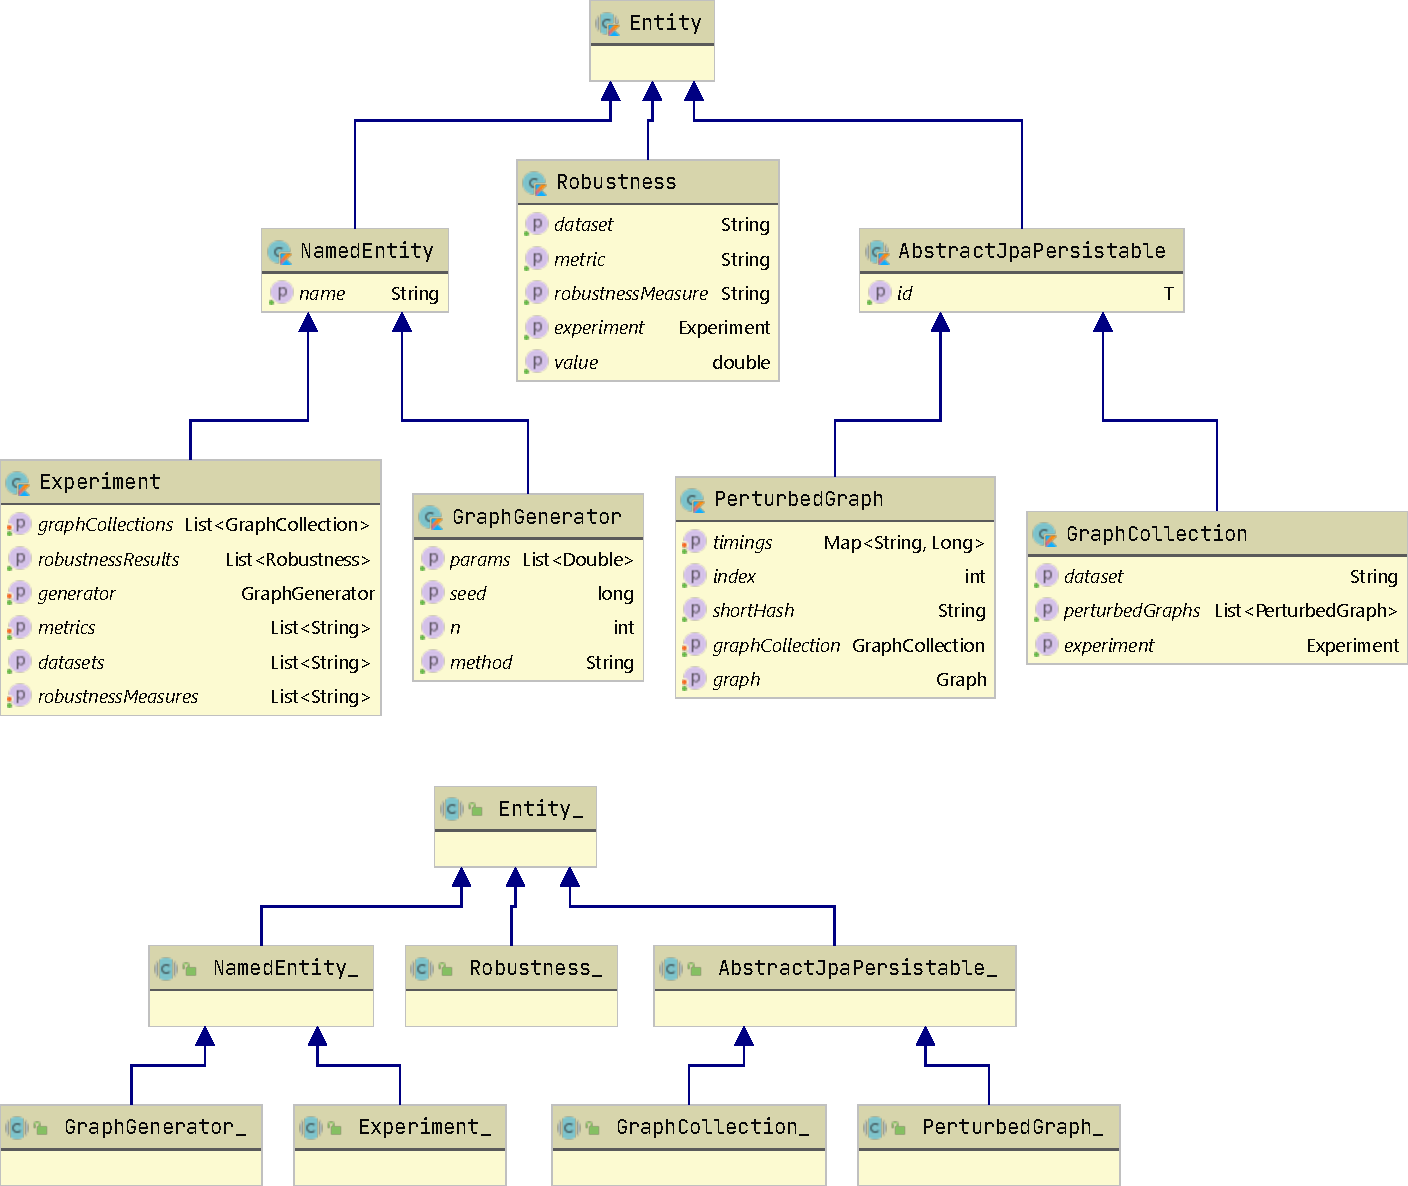
\includegraphics[width=\linewidth]{data_model_classes_diagram.pdf}
\caption{Inheritance hierarchy of the (Kotlin) classes underlying the persistence model presented in \autoref{fig:data_model_diagram}.
The arrows indicate \textsl{inheritance} (``is a'') relationships between classes.}
\label{fig:data_model_classes_diagram}
\end{figure}


Further, \autoref{fig:data_model_classes_diagram} shows the underlying \textsl{entity classes} written in Kotlin that have the following functions:
\begin{itemize}[topsep=5pt,label=$\bm{\rightarrow}$]
    \item \textbf{Data model definition}, seen in \autoref{fig:data_model_diagram}

    JPA provides a number of Java annotations to define entities (\texttt{@Entity}), their fields (\texttt{@Column}), constraints such as foreign key constraint (\texttt{@OneToMany}, \texttt{@ManyToOne} and others), and metadata such as rules for fetching data from database (e.g. \texttt{@Basic(fetch = FetchType.LAZY)} for lazy fetching of a field).
    Data model is inferred from these annotations that are processed during compile time

    Hibernate then abstracts away also operations such as creating and updating the database schema, which are configured in the \texttt{hibernate.cfg.xml} file (for example it creates a database from scratch if it doesn't exist).

    See \autoref{lst:kotlin_experiment_entity} for an example entity class using the JPA annotations.

    \item \textbf{Metamodel generation}

    Taking the annotated entity classes during compile time, Hibernate generates a \textsl{metamodel} class for each entity to allow writing type-safe queries.
    For example, the \texttt{Experiment\_} class is generated from the \texttt{Experiment} entity, with corresponding fields (such as \texttt{Experiment\_.name} of type \texttt{SingularAttribute<NamedEntity, String>}, or \texttt{Experiment\_.generator} of type \texttt{SingularAttribute<Experiment, GraphGenerator>}).

    See \autoref{lst:jpa_typed_query} for an illustration how generated metamodel classes aid in writing type-safe queries.

    \lstinputlisting[label={lst:jpa_typed_query}, linerange=jpa_typed_query0-jpa_typed_query1, caption={A toy example of using typed JPA queries. Note the \texttt{Experiment\_} metamodel class generated by Hibernate with (meta)fields corresponding to entities' fields}, float, language=Kotlin]{listings.kts}

    \item \textbf{Object-relational mapping}

    The classes (\autoref{fig:data_model_classes_diagram}) themselves carry the data managed by Hibernate.
    This means that other modules such as \texttt{generators} and \texttt{robustness} can use entity classes, while they are also managed by Hibernate.

    Hibernate is responsible for loading data into entity objects as well as persisting such objects.
    See \autoref{lst:hibernate_load_entity} for an illustration.

    \lstinputlisting[label={lst:hibernate_load_entity}, linerange=hibernate_load_entity0-hibernate_load_entity1, caption={A toy example of Hibernate loading and persisting an \texttt{Experiment} object.}, float, language=Kotlin]{listings.kts}
\end{itemize}


\autoref{lst:kotlin_experiment_entity} presents a full code listing of the \texttt{Experiment} entity.

\lstinputlisting[label={lst:kotlin_experiment_entity}, caption={The \texttt{Experiment} class written in Kotlin. Note especially the annotations which are enough to define the JPA data model.}, float, firstline=11,language=Kotlin]{Experiment.kt}

\subsection{H2 Database}

I employed the H2 relational database~\cite{MuellerH2DatabaseEngine2006} (based on SQL language) for storing entities, considering the following:
\begin{itemize}[topsep=5pt]
    \item Very fast; small footprint
    \item Easily embeddable, as it implements the JDBC API (Java Database Connectivity API, used by Hibernate too)
    \item Supports in-memory databases (good for testing)
    \item Written purely in Java, so can be bundled in \graffs and thus requires no other database installation in the client OS
\end{itemize}

\subsubsection*{Storing graphs in database}

Considering exporting graphs to various formats, I chose to store them purely as serialised \texttt{Graph} objects, including: \texttt{Node}s, \texttt{Edges}, and their attributes.


\section{Main pipeline}\label{sec:main_pipeline}

In this section I explain the steps of \graffs involved in calculating robustness measures of metrics.
In summary, the normal steps are:
\begin{enumerate}
    \item \textbf{Obtain datasets}, for example use demo datasets downloadable by the \graffs tool or provide any custom datasets
    \item \textbf{Define graph generator}, i.e. a way to generate new graphs from these datasets
    \item \textbf{Define an experiment} specifying a set of datasets to start with, a graph generator to use, a set of metrics to asses, and a set of robustness measures to evaluate stability of those metrics.
    \item \textbf{Run the experiment} computation (a computationally intensive task, which may, depending on the inputs and the environment, run in the order of magnitude of hours)

    This encompasses the following:
    \begin{enumerate}[label=\alph*.]
        \item \textbf{Generate perturbed graphs} (according to \autoref{sec:perturbing_graphs})
        \item \textbf{Calculate metric values} on the generated graphs, i.e. calculating a real number ($\mathbb{R}$) for each metric for each node in each generated graph (according to \autoref{sec:evaluating_metrics}).
        \item \textbf{Calculate robustness measures} for each metric, on collated perturbed graphs of each dataset
    \end{enumerate}
\end{enumerate}

All results, namely generated graphs with nodes including calculated values of each metric, and robustness measure results, are then stored in the database.

\begin{figure}
    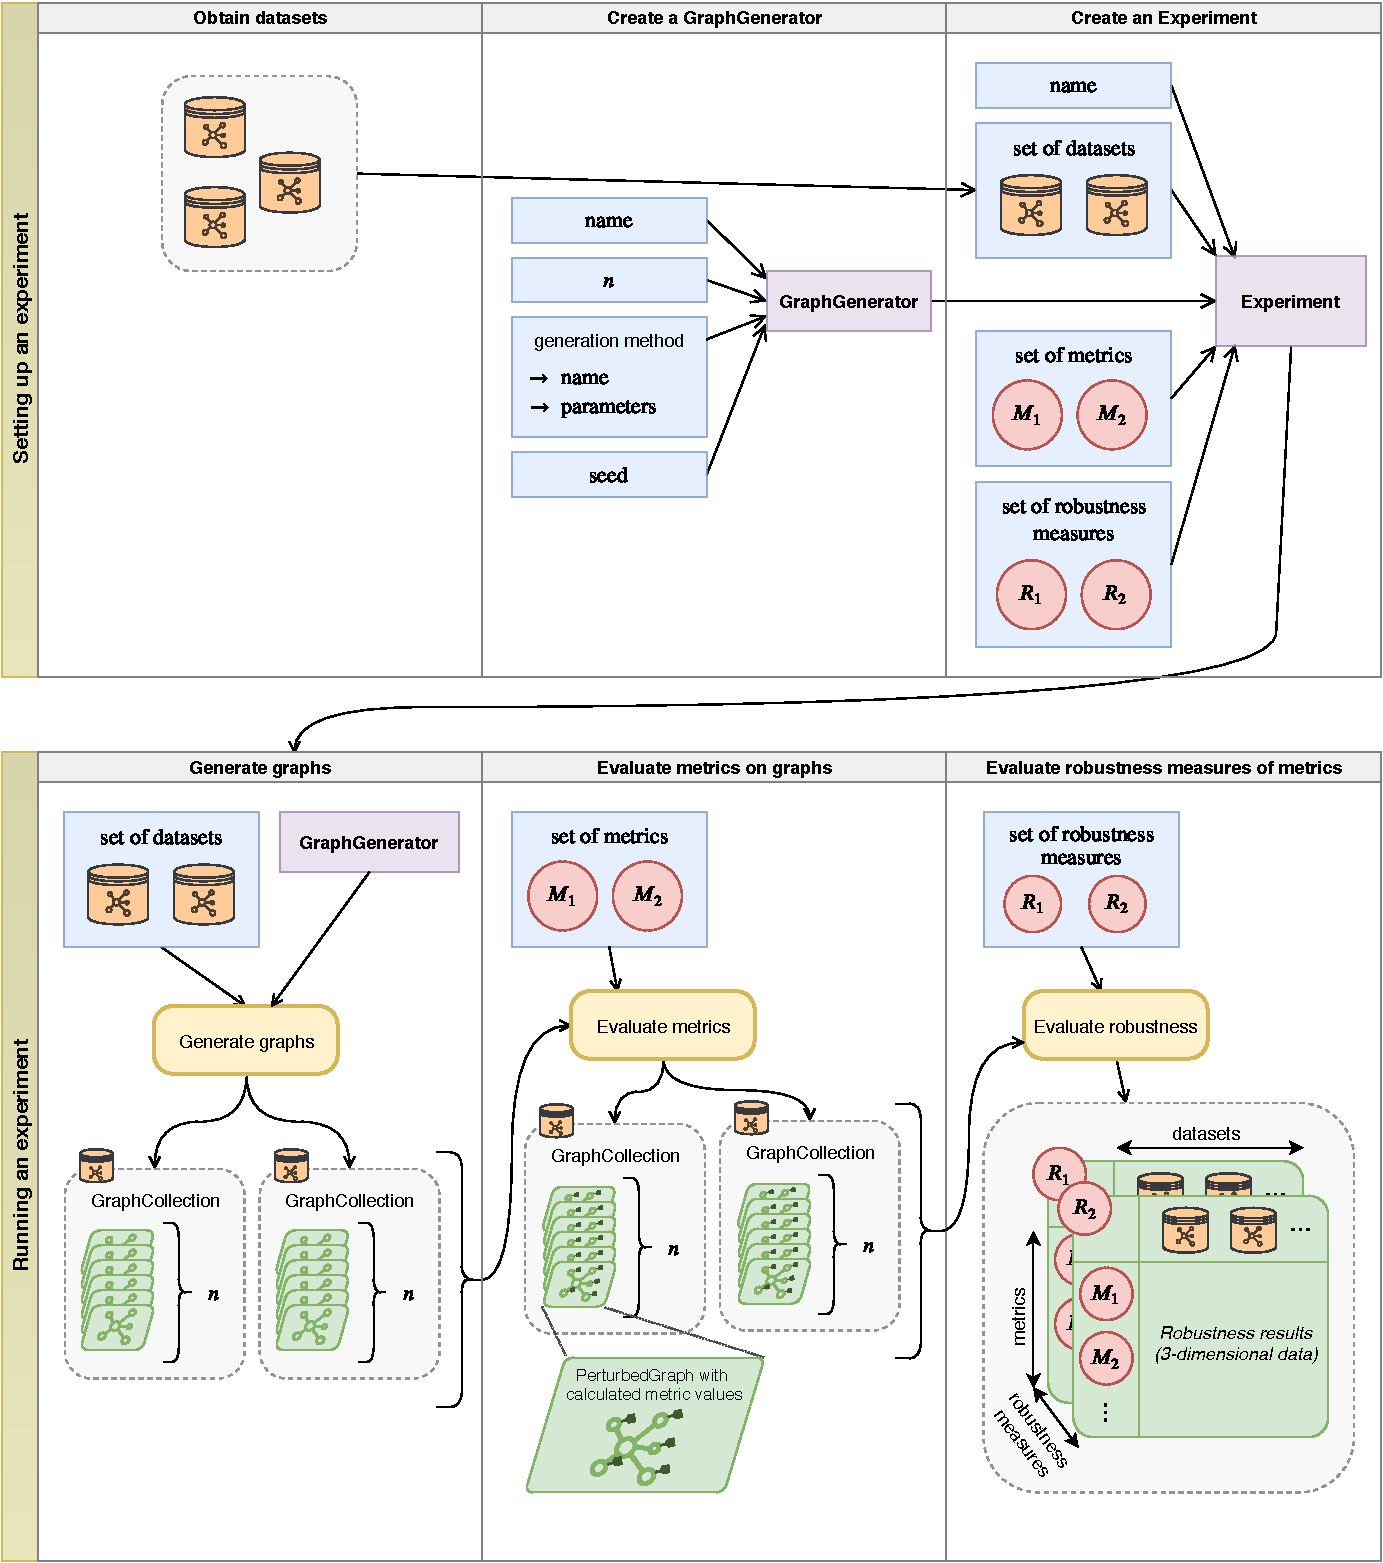
\includegraphics[width=\linewidth]{main_data_flow.pdf}
    \definecolor{diag-orange}{HTML}{D1A77D}
    \definecolor{diag-blue}{HTML}{6C8EBF}
    \definecolor{diag-violet}{HTML}{9673A6}
    \definecolor{diag-red}{HTML}{B85450}
    \definecolor{diag-yellow}{HTML}{D6B656}
    \definecolor{diag-green}{HTML}{82B366}
    \caption{Diagram showing the data flow of an experiment, in two phases: 1. setting up an experiment (the user collects/inputs data), 2. running an experiment (the program is running the computations as described in \autoref{sec:main_pipeline}). The result is a 3-dimensional data with a calculated robustness value for each from \textsl{datasets, metrics, robustness measures}.}\label{fig:main_data_flow}
    \footnotesize\justify\vspace{-0.4\baselineskip}
    Legend: \textcolor{diag-orange}{orange} -- datasets; \textcolor{diag-blue}{blue} -- user input; \textcolor{diag-violet}{violet} -- user-defined persisted entity; \textcolor{diag-red}{red} -- program-defined operations; \textcolor{diag-yellow}{yellow} -- processes; \textcolor{diag-green}{green} -- program-generated output; arrows $\rightarrow$ represent the flow of data.
\end{figure}


Running the experiment is a computationally intensive task, mainly due to metric evaluation (which certainly depends on the chosen metrics).
To mitigate this, I employed the following:
\begin{itemize}[topsep=5pt]
    \item Optimised the program for computation speed by applying performance engineering principles \todo{elaborate}
    \item Allow parallel computation
    \item I ran extensive experiments on a high-performance computing facility (from \autoref{sec:computing_cluster})
\end{itemize}

\autoref{fig:main_data_flow} illustrates the flow of data across the above-mentioned steps.

\subsection{Loading datasets}

Datasets are located, and are expected to be located, in the `data' directory in the \graffs's working directory (i.e. where the program is run).
Each sub-directory represents a dataset identified by the sub-directory's name.
\graffs supports loading files of two different types of files:

\begin{description}
    \item \hyperref[sec:edge_files]{\textbf{Edge files}} -- text format with each line containing a pair of adjacent nodes
    \item \hyperref[sec:rdata_files]{\textbf{\texttt{RData} files}} -- binary files that store objects created in the R language~\cite{RCoreTeamLanguageEnvironmentStatistical2009}
\end{description}

\begin{figure}
\begin{tikzpicture}%
\draw[color=black!60!white]
\FTdir(\FTroot,i0,data){
\FTdir(i0,i1,citation){
\FTfile(i1,edges.txt)
\FTfile(i1,info.txt)
}
\FTdir(i0,i2,ecoli){
\FTfile(i2,info.txt)
\FTfile(i2,string\_ecoli\_data.RData)
}
\FTdir(i0,i3,facebook){
\FTfile(i3,edges.txt)
\FTfile(i3,info.txt)
}
\FTdir(i0,i4,pvivax){
\FTfile(i4,info.txt)
\FTfile(i4,string\_pvivax\_data.RData)
}
\FTdir(i0,i5,test){
\FTfile(i5,edges.txt)
}
\FTdir(i0,i6,yeast){
\FTfile(i6,info.txt)
\FTfile(i6,string\_yeast\_data.RData)
}
};
\end{tikzpicture}

\caption{An example structure of the \texttt{data} directory}
\label{fig:data_dir_structure}
\end{figure}


In each dataset's directory, the program looks for a file that ends with either \texttt{.RData} or \texttt{.txt}, in this order.
Datasets may additionally contain an \texttt{info.txt} file holding a human-readable description of the dataset (that is printed in the command-line interface when the dataset is loaded).
\autoref{fig:data_dir_structure} shows an example directory structure.

The \texttt{GraphLoader} abstract class (\autoref{lst:code_graphloader}) is to be implemented in both cases.
\lstinputlisting[label={lst:code_graphloader}, caption={The \texttt{GraphLoader} abstract class, providing a contract for implementations to load graphs}, float=h, language=Kotlin, firstline=6]{GraphLoader.kt}

\subsubsection{Edge files}\label{sec:edge_files}

A common pure format of storing network structure (without any metadata) is to list the edges line by line, with each line containing unique identifiers of two nodes.
The set of nodes is then implicitly defined by the set of all distinct node identifiers present in the file.

However, different dataset sources (\autoref{sec:datasets}) provide \texttt{.txt} edge files with the content in different formats.
Some edge files contain a header, \texttt{\#comments}, or a third number in each line representing the edge's weight (for \hyperref[sec:scored_networks]{scored networks}).
\autoref{fig:edge_file_examples} shows a number of example edge files that should be accepted by \graffs.

%! Suppress = Ellipsis
% @formatter:off
\begin{savenotes}
\begin{figure}[!ht]
\caption{Three examples of dataset files containing one edge definition per line.}\label{fig:edge_file_examples}
\begin{minipage}[t]{.12\textwidth}
\raggedright\footnotesize \texttt{edges.txt}, a~sample graph file
\begin{lstlisting}
0 1
0 2
0 3
0 4
0 5
0 6
0 7
1 2
1 4
1 5
1 8
1 9
1 10¦\Suppresslinenumbers¦
...
\end{lstlisting}\Reactivatelinenumbers
\end{minipage}\hspace*{0.8cm}%
\begin{minipage}[t]{.36\textwidth}
\footnotesize \texttt{Cit-HepTh.txt} citation network from Stan\-ford Large Network Data\-set Col\-lec\-tion\footnote{URL: \url{https://snap.stanford.edu/data/cit-HepTh.html}}
\begin{lstlisting}
# Directed graph (each unordered pair of nodes is saved once): Cit-HepTh.txt
# Paper citation network of Arxiv High Energy Physics Theory category
# Nodes: 27770 Edges: 352807
# FromNodeId	ToNodeId
1001	9304045
1001	9308122
1001	9309097
1001	9311042
1001	9401139¦\Suppresslinenumbers¦
...
\end{lstlisting}\Reactivatelinenumbers
\end{minipage}\hspace*{0.8cm}%
\begin{minipage}[t]{0.41\textwidth}
\footnotesize \texttt{362663.protein.links.v11.0.txt} \\(Escherichia coli) from the STRING data\-base\footnote{URL: \url{https://string-db.org/cgi/download.pl?species_text=Escherichia+coli+536}}
\begin{lstlisting}
protein1 protein2 combined_score
362663.ECP_0001 362663.ECP_0006 518
362663.ECP_0001 362663.ECP_0003 606
362663.ECP_0001 362663.ECP_0002 606
362663.ECP_0001 362663.ECP_0005 518
362663.ECP_0001 362663.ECP_0004 606
362663.ECP_0002 362663.ECP_0798 158
362663.ECP_0002 362663.ECP_1284 175
362663.ECP_0002 362663.ECP_1357 170
362663.ECP_0002 362663.ECP_0918 621
362663.ECP_0002 362663.ECP_1773 175
362663.ECP_0002 362663.ECP_2824 342
362663.ECP_0002 362663.ECP_4415 320¦\Suppresslinenumbers¦
...
\end{lstlisting}\Reactivatelinenumbers
\end{minipage}%
\hspace*{-0.5cm}
\end{figure}
\end{savenotes}
% @formatter:on


One way would be to distinguish different formats by the file extension, or with additional meta information.
However, one of the goals for \graffs is to make it as versatile as possible, thus not requiring the user to manually specify a dataset's type or source is welcome.

Hence, I implemented \texttt{FileSourceEdgeOptionalWeight} parser, extending GraphStream's \texttt{FileSourceEdge} simple LR parser, to allow the following:
\begin{itemize}[topsep=5pt]
    \item Modify the grammar to correctly parse node IDs containing dots (\texttt{.}), such as \texttt{362663.ECP\_0001} (to allow datasets from the STRING database)
    \item Ignore comment lines starting with \texttt{\#} or \texttt{\%} characters
    \item Ignore headers starting with the string \texttt{protein1} (included in graph files downloaded from the STRING database)
    \item Recognise if a line has 3 tokens instead of 2, in which case parse and store it as the weight of the edge
\end{itemize}

\subsubsection{RData files}\label{sec:rdata_files}

The Paper\cite{Bozhilova2019} provides the dataset files that were used in their research\footnote{Available at \url{http://opig.stats.ox.ac.uk/resources}}, in the \texttt{RData} format, a binary file capturing a session of the R language, storing objects from the \texttt{igraph} R package.

To load such files, an option is to convert them manually into another \graffs-readable format, or let \graffs call R to do this conversion under the hood.
To make \graffs as versatile as possible and not require the R software environment to be installed on the client's computer, I employed the Renjin library\footnote{Rejin official website: \url{https://www.renjin.org/}}, a \enquote{JVM-based interpreter for the R programming language}.
Renjin can execute R code (as well as load RData files) within Java, without the need to install any additional platform.

When an RData file is to be loaded in \graffs, a Renjin engine starts under the hood and loads desired file.
If an object whose name ends with \texttt{.df}\footnotemark{} is found, it is converted into a GraphStream's \texttt{Graph} object.
\footnotetext{This is to follow convention from \url{https://github.com/lbozhilova/measuring_rank_robustness/blob/c39bfed/data_prep.R}}

\subsection{Generating graphs}

First, there is the \texttt{GraphProducer} interface, which has a single method\footnotemark{}:\\ \texttt{fun produce(sourceGraph: Graph, n: Int): List<Deferred<PerturbedGraph>>}
\footnotetext{It returns a list of \texttt{Deferred} objects from the \texttt{kotlinx.coroutines} package, so that the generation can be parallelised at a higher level in the program using \textsl{Kotlin coroutines}, as described in \autoref{sec:kotlin_coroutines}.}
Each |GraphProducer| implementation also provides a corresponding |GraphProducerFactory| object, defined as:
% @formatter:off
\begin{lstlisting}[language=Kotlin]
typealias GraphProducerFactory =
    (seed: Long, params: List<Number>, coroutineScope: CoroutineScope) -> GraphProducer
\end{lstlisting}
% @formatter:on

Further, \texttt{GraphGenerator}s (from \autoref{fig:data_model_classes_diagram}), which are stored in the database, have the \texttt{method} field referencing a \texttt{GraphProducer} to use.

Implementations of the methods for producing graphs as described in~\autoref{sec:perturbing_graphs} are straightforward.
Each generated graph is in some way a copy of the input graph, with some edges deleted.

\subsection{Evaluating metrics}

Metrics are classes (or rather, Kotlin |object|s) implementing the |Metric| interface, with a single method \texttt{fun evaluate(graph: Graph): MetricResult?}.

In the database, each |PerturbedGraph| entry stores a single serialised |Graph| object, whose nodes holds values for all metrics.
A metric's value at each node is stored in the node's attribute map.

An |Experiment| entry (those are created by the user) has a |Set<String>| field specifying which metrics to evaluate on each |PerturbedGraph|, and those metrics are again referenced by a |String| identifier.

\subsection{Metric robustness}

Similar to other concepts, robustness measures are classes implementing the |RobustnessMeasure| interface, with a single method |suspend fun evaluate(metric: MetricInfo, graphCollection: GraphCollection, metadata: GraphCollectionMetadata): Double|.

|MetricInfo| uniquely identifies the |Metric| whose robustness to calculate.
|GraphCollection| is an entity (from \autoref{fig:data_model_classes_diagram}) with a list of |PerturbedGraph|s of one dataset.
|GraphCollectionMetadata| provides cached\footnotemark{} access to intermediate results regarding the particular |GraphCollection| in the context of the current |Metric|, such as the overall ranking of the given metric over all the perturbed graphs (see Definition~\ref{def:overall_ranking}).
\footnotetext{cached, as the overall ranking is calculated only once for each \texttt{GraphCollection} and each \texttt{Metric}, and used for more robustness measures}
Each |RobustnessMeasure| returns a single |Double| value, which is the numerical result, calculated as described in \autoref{sec:robustness_measures}.
The |evaluate| function has the |suspend| modifier so that it can suspend and finish asynchronously within the context of Kotlin coroutines (see \autoref{sec:kotlin_coroutines}).

\subsection{Visualising graphs & producing figures}

\todo{todo}


\section{Parallelism using Kotlin coroutines}
\label{sec:kotlin_coroutines}

Kotlin supports a concept of \textsl{suspending functions}, i.e. functions which can pause their execution (storing its \textsl{current continuation}) and return the control of the flow back to its caller, and later continue by resuming the continuation at the suspension point.
The context in which a suspending function suspends, is called coroutine.
Coroutines are a well-known control abstraction in programming languages\cite{MouraRevisitingCoroutines2009} that can easily be implemented in higher-order languages using continuations\cite{HaynesContinuationsCoroutines1984}.

Asynchronous computations, delays, or IO operations can be programmed as suspending calls, i.e. functions that are allowed to \textsl{suspend} (or \textsl{pause}) coroutine voluntarily, and return the control back to the caller, then continue whenever their \textsl{continuation} is resumed (or invoked).

Coroutines can be used even within a single thread, and so allow a concurrent execution.
In the case of \graffs, however, we are interested in running computation in parallel, to utilise the power of multiple CPU cores.
A simple solution in Java would be to use |Thread|s, or a library working with threads directly.
This would work but it's heavyweight, not very expressive and not safe (e.g. a failure of an operation in one thread will not automatically cancel following or related tasks in other threads, unless this safety is implemented manually).
Another option is to use job queueing and an abstract multi-threaded executor, but then specifying inter-task execution order constraints would still be verbose, and running jobs would not be abstracted away from the code defining the jobs.

Kotlin coroutines are \textsl{lightweight threads} -- spawning coroutines is fast and cheap\cite{AriasFunctionalKotlinExtend2018}.
They have a similar life cycle and are executed within regular threads, although they are not bound to them\cite{TorresLearningConcurrencyKotlin2018}.
Coroutines allow executing suspending functions.

Suspending functions in Kotlin, when compiled to Java bytecode, are regular functions accepting |Continuation<Int>| as one of the arguments.
The |async| function (or its alternatives) takes a suspending function, creates an asynchronous coroutine executing the function and immediately returns its future result (as |Deferred<T>|).
Then the |await| suspending function called on a |Deferred| object waits for the resulting value without blocking, and resumes when the deferred computation is complete.

Kotlin also provides other means to synchronise coroutines, such as using mutual exclusion or actors, when needed in a parallel execution.
Mutexes are used to ensure synchronised access when persisting entities in the database.

\todo{diagram similar to \url{https://s3.amazonaws.com/kukuruku-co/uploads/images/00/17/75/2016/10/09/126426.png}}

The following parts of \graffs use parallel programming with coroutines:
\begin{itemize}[topsep=5pt]
    \item Generating graphs
    \item Evaluating metrics on graphs

    Each |Graph| is treated individually without the need to synchronise across them, however, evaluation of metrics within one |Graph| is sequential as the GraphStream library does not support parallel access.
    \item Evaluating robustness, including calculating overall ranks, which must be calculated for each |GraphCollection| before any robustness measure is evaluated on it
    \item Generating various figures, for which an intermediate
\end{itemize}


\section{Command line interface}\label{sec:cli}

The \graffs tool is built as a program with rich and intuitive command-line interface.
The program is pre-packaged in a \texttt{.jar} file, built for Java 8 or higher, so running it involves running the shell command:
% @formatter:off
\begin{lstlisting}[language=bash,style=light]
java -jar graffs.jar [ARGS]
\end{lstlisting}
% @formatter:on

Clikt\citeneeded is a \enquote{multiplatform command line interface parsing for Kotlin} library that I used for defining commands, their behaviour, description, and hierarchy, in a structured way.
The library utilises a number of features of the Kotlin language, such as delegated properties, extension functions, and default arguments, resulting in a cleaner code that uses the library.

The \graffs tool provides many commands (loading datasets, creating and accessing graph generators, creating and running experiments, and so on).
Commands are grouped based on their context and the objects that they operate on, and can further have sub-commands.
Those are together structured in a tree-like hierarchy.
The hierarchy is shown in \autoref{fig:cli_commands_hierarchy}.

\begin{figure}
\caption{Hierarchy of supported command-line interface commands, and their brief description}
\label{fig:cli_commands_hierarchy}
\begin{flushleft}
\setlength{\DTbaselineskip}{11pt}
\small
\dirtree{%
.1 graffs \scriptsize \dotfill\ \begin{minipage}[t]{10.6cm}Tool for evaluating Graph Metric Robustness\end{minipage}.
.2 dataset \scriptsize \dotfill\ \begin{minipage}[t]{10.6cm}Access available datasets\end{minipage}.
.3 list \scriptsize \dotfill\ \begin{minipage}[t]{10.6cm}List all datasets available in the `data` directory\end{minipage}.
.3 load \scriptsize \dotfill\ \begin{minipage}[t]{10.6cm}Check if datasets can be loaded from the `data` directory\end{minipage}.
.3 download-demos \scriptsize \dotfill\ \begin{minipage}[t]{10.6cm}Download datasets for demonstration\end{minipage}.
.3 viz \scriptsize \dotfill\ \begin{minipage}[t]{10.6cm}Visualise graph\end{minipage}.
.2 metric \scriptsize \dotfill\ \begin{minipage}[t]{10.6cm}Access available metrics\end{minipage}.
.3 list \scriptsize \dotfill\ \begin{minipage}[t]{10.6cm}List available graph metrics\end{minipage}.
.2 generator \scriptsize \dotfill\ \begin{minipage}[t]{10.6cm}Create or list graph generators\end{minipage}.
.3 list \scriptsize \dotfill\ \begin{minipage}[t]{10.6cm}List available graph generators\end{minipage}.
.3 create \scriptsize \dotfill\ \begin{minipage}[t]{10.6cm}Create a new graph generator description\end{minipage}.
.3 remove \scriptsize \dotfill\ \begin{minipage}[t]{10.6cm}Remove a graph generator\end{minipage}.
.2 experiment \scriptsize \dotfill\ \begin{minipage}[t]{10.6cm}Manage experiments (evaluating metrics on generated graphs)\end{minipage}.
.3 list \scriptsize \dotfill\ \begin{minipage}[t]{10.6cm}List created experiments and their properties\end{minipage}.
.3 create \scriptsize \dotfill\ \begin{minipage}[t]{10.6cm}Create an experiment\end{minipage}.
.3 change \scriptsize \dotfill\ \begin{minipage}[t]{10.6cm}Change an existing experiment\end{minipage}.
.3 clone \scriptsize \dotfill\ \begin{minipage}[t]{10.6cm}Create a new experiment using parameters of existing experiment\end{minipage}.
.3 remove \scriptsize \dotfill\ \begin{minipage}[t]{10.6cm}Remove an experiment, all its generated graph and any computed results\end{minipage}.
.3 run \scriptsize \dotfill\ \begin{minipage}[t]{10.6cm}Run an experiment\end{minipage}.
.3 prune \scriptsize \dotfill\ \begin{minipage}[t]{10.6cm}Remove generated graphs and calculated robustness values of an experiment\end{minipage}.
.2 plot \scriptsize \dotfill\ \begin{minipage}[t]{10.6cm}Plot results\end{minipage}.
.3 rank-similarity.
.2 db \scriptsize \dotfill\ \begin{minipage}[t]{10.6cm}Manage the underlying database\end{minipage}.
.3 test \scriptsize \dotfill\ \begin{minipage}[t]{10.6cm}Test the database connection\end{minipage}.
.3 drop \scriptsize \dotfill\ \begin{minipage}[t]{10.6cm}Reset the database schema and contents\end{minipage}.
}
\end{flushleft}
\end{figure}


Further, \autoref{lst:graffs_cli_examples} shows an example output of some of the commands.

\lstinputlisting[label={lst:graffs_cli_examples}, caption={A demonstration of the help text printed by the command-line tool}, float, basicstyle=\ttfamily\color{black}\fontsize{8pt}{8pt}\selectfont,]{graffs-help.txt}

\todo{Describe Clikt features such as command completion}

\section{Testing}

\subsection{Unit testing}
Using JUnit 5

\subsection{Continuous Integration}
CircleCI


\section{Documentation}

The Kotlin code is documented using the \texttt{KDoc} language and an HTML documentation is generated using the \texttt{Dokka} tool (similar to \texttt{JavaDoc}).\citeneeded

I wrote the documentation in code most thoroughly for public classes, and their members that need clarification on their behaviour or usage.



